%% %% %% %%
%%
%% Parte A de la práctica
%%
%% %% %% %%

\documentclass[../procedimientos.tex]{subfiles}
\graphicspath{{\subfix{../../images/}}}

\begin{document}
\clearpage
\subsection{Parte A}
\begin{em}
  Diseñar mediante programación estructurada la implementación de un sumador
  binario de dos palabras de 4 bits.
\end{em}
\begin{figure}[H]
  \centering
  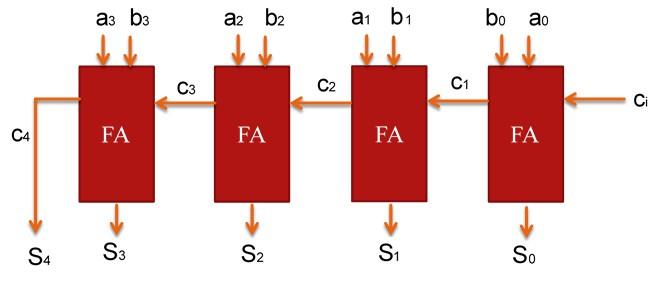
\includegraphics[width=0.6\textwidth]{inciso-a}
  \caption{Circuito de ejemplo (Parte A)}
  \label{fig:inciso_a}
\end{figure}

Para comenzar, primero se debe implementar el componente \textit{Full Adder 
(FA)}. El cual se comporta según la siguiente tabla de verdad.
\begin{table}[h]
  \centering
  \begin{tabular}{ccc|cc}
    $a$ & $b$ & $c$ & $s$ & $c_o$\\
    \hline
    0 & 0 & 0 & 0 & 0\\
    0 & 0 & 1 & 1 & 0\\
    0 & 1 & 0 & 1 & 0\\
    0 & 1 & 1 & 0 & 1\\
    1 & 0 & 0 & 1 & 0\\
    1 & 0 & 1 & 0 & 1\\
    1 & 1 & 0 & 0 & 1\\
    1 & 1 & 1 & 1 & 1\\
  \end{tabular}
  \caption{Tabla de verdad de un \textit{Full Adder}}
\end{table}

Obteniendo las expresiones para el cálculo de $s$ y $c_o$, se tiene que:
\begin{align*}
  s(abc)  &= \sum_m (1,2,4,7)\\
            &= \n{a}\n{b}c + \n{a}b\n{c} + a\n{b}\n{c} + abc\\
            &= \n{a}(\n{b}c + b\n{c}) + a(\n{b}\n{c} + bc)\\
            &= \n{a}(b \oplus c) + a \overline{(b \oplus c)}\\
            &= a \oplus (b \oplus c)
\end{align*}
\begin{equation*}
  \boxed{
    \therefore s(abc) = a \oplus (b \oplus c)
  }
\end{equation*}

Por otra parte, se tiene que:
\begin{align*}
  c_o(abc)  &= \sum_m (3,5,6,7)\\
            &= \n{a}bc + a\n{b}c + ab\n{c} + abc\\
            &= c(\n{a}b + a\n{b}) + ab\cancel{(\n{c}+c)}\\
            &= c(a \oplus b) + ab
\end{align*}
\begin{equation*}
  \boxed{
    \therefore c_o(abc) = c(a \oplus b) + ab
  }
\end{equation*}

De esta forma, a través del uso del lenguaje \textit{VHDL}, se implementó la 
entidad \texttt{FA}, la cual toma un vector de entrada \texttt{ent} y un 
vector de salida \texttt{res}.

\begin{lstlisting}[language=VHDL]
-- Implementacion: Full Adder (Parte A)
entity FA is
	port(
    ent	:in	  std_logic_vector(2 downto 0);
		res	:out	std_logic_vector(1 downto 0)
	);
end entity;

architecture Behave of FA is
	signal a, b, ci	:std_logic;
begin
  a   <= ent(2);
  b   <= ent(1);
  ci  <= ent(0);
  res <= (
    a xor b xor ci,
    (ci and (a xor b)) or (a and b)
  );
end;
\end{lstlisting}

El vector de entrada de \texttt{ent} se representa de la siguiente forma:
\begin{itemize}
  \item $a \rightarrow ent(2)$
  \item $b \rightarrow ent(1)$
  \item $c \rightarrow ent(0)$
\end{itemize}

Mientras que las salidas \texttt{res} se representa de la siguiente forma:
\begin{itemize}
  \item $s \rightarrow res(1)$
  \item $c_o \rightarrow res(0)$
\end{itemize}

Posteriormente, se hizo la integración completa del sumador binario de dos 
palabras de 4 bits en una nueva entidad, la cual se llamó \texttt{Adder4}. Es 
importante considerar que se debe de realizar la operación en forma de cadena.
\begin{itemize}
  \item Para el bit 0, se toma como entrada $a(0)$, $b(0)$ y $ci$. Se devuelve 
    el primer bit del resultado $s(0)$ y un bit de acarreo, el cual se 
    almacena dentro de una señal $c(0)$.
  \item Para el bit 1, se toma como entrada $a(1)$, $b(1)$ y $c(0)$. Se 
    devuelve el segundo bit del resultado $s(1)$ y un bit de acarreo, el cual 
    se almacena dentro de una señal $c(1)$.
  \item Para el bit 1, se toma como entrada $a(2)$, $b(2)$ y $c(1)$. Se 
    devuelve el segundo bit del resultado $s(2)$ y un bit de acarreo, el cual 
    se almacena dentro de una señal $c(2)$.
  \item Para el bit 1, se toma como entrada $a(3)$, $b(3)$ y $c(2)$. Se 
    devuelve el segundo bit del resultado $s(3)$ y un bit de acarreo, a su vez 
    conforma el bit más significativo del resultado, que se almacena 
    directamente en $s(4)$.
\end{itemize}

Lo anterior se resume en la siguiente entidad:
\begin{lstlisting}[language=VHDL]
-- Implementacion: Suamador 4 bits (Parte A)
entity Adder4 is
	port(
		a,b		:in std_logic_vector(3 downto 0);
    ci		:in std_logic;
		s			:out std_logic_vector(4 downto 0)
	);
end;

architecture Behave of Adder4 is
	component FA is
		port(
			ent	:in	std_logic_vector(2 downto 0);
			res	:out	std_logic_vector(1 downto 0)
		);
	end component;
  signal c :std_logic_vector(2 downto 0);
begin
  adder_0	:FA port map(
		ent => (a(0), b(0), ci),
		res(1) => s(0),
		res(0) => c(0)
	);
  adder_1	:FA port map(
		ent => (a(1), b(1), c(0)),
		res(1) => s(1),
		res(0) => c(1)
	);
  adder_2	:FA port map(
		ent => (a(2), b(2), c(1)),
		res(1) => s(2),
		res(0) => c(2)
	);
  adder_3	:FA port map(
		ent => (a(3), b(3), c(2)),
		res(1) => s(3),
		res(0) => s(4)
	);
end;
\end{lstlisting}

\subsubsection*{Ejecución en Quartus II}
Para comprobar el funcionamiento del circuito implementado, se puede realizar 
una simulación a través de un archivo \textit{University Program VWF}. Se 
realizaron 16 casos en los que los valores de $a$ se generaron 
secuencialmente, mientras que los valores de $b$ se generaron de forma 
aleatoria. Los primeros ocho casos de prueba tienen $c_i = 0$, y los demás 
tienen $c_i = 1$. El resultado es el siguiente:
\begin{figure}[H]
  \centering
  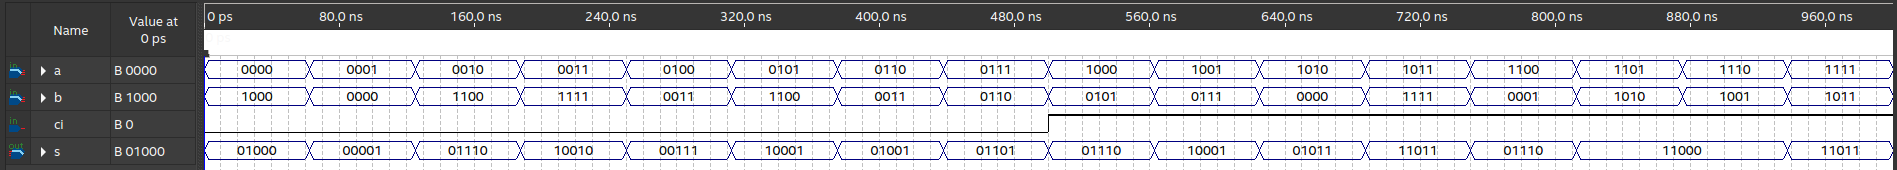
\includegraphics[width=\textwidth]{inciso-a-sim}
  \caption{Simulación del circuito (Parte A)}
  \label{fig:inciso_a_sim}
\end{figure}

En la Figura \ref{fig:inciso_a_sim} se puede comprobar el correcto 
funcionamiento del sumador.

Es importante recalcar el uso de las nuevas herramientas que vimos en clase.  
Primero, se puede ver la utilización de una entidad dentro de otra entidad 
(como es el caso de \texttt{FA} dentro de \texttt{Addder4}). Fue importante 
utilizar la declaración del componente \textit{FA} dentro de \texttt{Adder4} 
(similar a una importación en otros lenguajes de programación). Se deben crear 
varias instanicias de este mismo tipo (\texttt{adder\_0}, \texttt{adder\_1}, 
\texttt{adder\_2} y \texttt{adder\_3}), cada una de las cuales se encarga de 
calcular un bit en específico. Para poder declarar cada una de ellas de forma 
adecuada, es necesario hacer un mapeo de puertos a través de la instrucción 
\texttt{port map}. En la cual se tienen que asignar los valores de las 
entradas y también, a través de este, se asignan las salidas.
\end{document}
